\documentclass{article}
\usepackage{listings}
\usepackage{color}
\usepackage{amsmath}
\usepackage{mathtools}
\usepackage{amsfonts}
\usepackage{amssymb}
\usepackage{caption}
\usepackage{tabularx}
\usepackage[export]{adjustbox}
\usepackage{polski}
\usepackage{indentfirst}
\usepackage{graphicx}
\usepackage{pdfpages}
\usepackage{float}
\usepackage{gauss}

\DeclareCaptionType{equ}[][List of equations]
\captionsetup[equ]{labelformat=empty}

%script adding bars in matrix
\usepackage{etoolbox}
\makeatletter
\patchcmd\g@matrix
 {\vbox\bgroup}
 {\vbox\bgroup\normalbaselines}% restore the standard baselineskip
 {}{}
\makeatother

\newcommand{\BAR}{%
  \hspace{-\arraycolsep}%
  \strut\vrule % the `\vrule` is as high and deep as a strut
  \hspace{-\arraycolsep}%
}
\definecolor{dkgreen}{rgb}{0,0.6,0}
\definecolor{gray}{rgb}{0.5,0.5,0.5}
\definecolor{mauve}{rgb}{0.58,0,0.82}

\lstset{frame=tb,
  language=Python,
  aboveskip=3mm,
  belowskip=3mm,
  showstringspaces=false,
  columns=flexible,
  basicstyle={\small\ttfamily},
  numbers=none,
  numberstyle=\tiny\color{gray},
  keywordstyle=\color{blue},
  commentstyle=\color{dkgreen},
  stringstyle=\color{mauve},
  breaklines=true,
  breakatwhitespace=true,
  tabsize=3,
  extendedchars=\true,
  inputencoding=utf8x
}

\lstset{literate={ą}{{\k{a}}}1 {ł}{{\l{}}}1 {ń}{{\'n}}1 {ę}{{\k{e}}}1 {ś}{{\'s}}1 {ż}{{\.z}}1 {ó}{{\'o}}1 {ź}{{\'z}}1 {Ą}{{\k{A}}}1 {Ł}{{\L{}}}1 {Ń}{{\'N}}1 {Ę}{{\k{E}}}1 {Ś}{{\'S}}1 {Ż}{{\.Z}}1 {Ó}{{\'O}}1 {Ź}{{\'Z}}1 }

\begin{document}
\title{Sprawozdanie - Metody numeryczne i optymailzacja}
\author{Jakub Andryszczak 259519,\\ Jakub Żak 244255,\\ Maciej Cierpisz 249163}
\date{}
\maketitle

\newpage
\tableofcontents
%Tutaj zaczyna się wstęp

\newpage
\section{Zadanie nr. 1}
Znajdź liczby x1 i x2, które maksymalizują sumę x1 + x2 przy ograniczeniach:
\begin{equation}
    \begin{cases}
      x_{1} \geq 0,x_{2}\geq 0 \\
     x_{1}+2x_{2} \leq 2 \\
     4x_{1} + 2x_{2}\leq 12\\
     -x_1 + x_2 \leq 1, 
    \end{cases}\,.
  \end{equation}
  Narysować zbiór dopuszczalnych rozwiązań na $\Re^2$ i znaleźć rozwiązanie w ujęciu
geometrycznym, formułując zadanie programowania liniowego.
\newline

Początkowo zapisano wszystkie nierówności w formie równań z dodatkową niewiadomą,
\begin{equation}
    \begin{cases}
      x_{1}+2x_{2}+x_3 = 2 \\
     4x_{1} + 2x_{2}+x_4 = 12\\
     -x_1 + x_2 + x_5 = 1, 
    \end{cases}
  \end{equation}
  Zapisano zadanie w postaci macierzowej:
  \begin{equation}
    \begin{gmatrix}[b]
      1&1&1&0&0&4\\
      4&2&0&1&0&12\\
      -1&1&0&0&1&1\\
      1&1&0&0&0&0
    \end{gmatrix}
  \end{equation}
Następnie wyświetlono wszystkie proste na jednym wykresie.\newpage
\begin{figure}[h]
    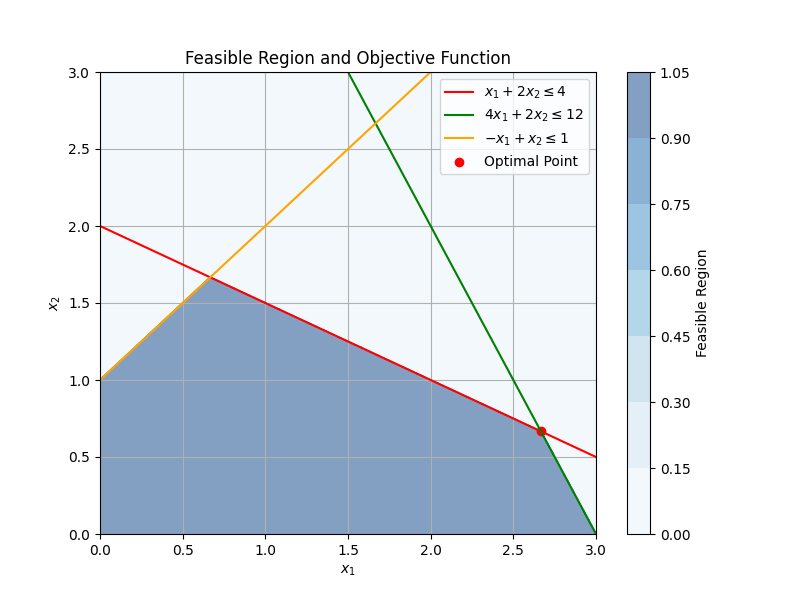
\includegraphics[scale=0.5]{Simplex1.png}
    \centering
    \captionsetup[Tabela]{name=New Table Name}
    \caption*{Wykres.2.1. Zależność n-tej iteracji metody do błędu residualnego}
  \end{figure}
  Obszar zamalowany jest zbiorem dopuszczalnych rozwiązań dla podanych warunków zadania.
  Liczby $x_1$ i $x_2$, które maksymalizują ich sumę przy podanych ograniczeniach są:
  \begin{equation}
    \begin{cases}
      x_1 = 2.6667\\
      x_2 = 0.6667\\
      f(x_1,x_2) = 3.3333
    \end{cases}
  \end{equation}
Kolejno zweryfikowano czy znalezione rozwiązanie jest poprawne. Do tego wykorzystano funkcję
linprog(.). Zauważono, że wyniki są spójne. Wykonano obliczenia również na samodzielnie wykonanej funkcji, aby porównać czas i dokładność względem funkcji linprog.
\newline
Czas w jakim została wykonana ręcznie wykonana funkcja bez wykorzystania linprog: 0.0004387 [s]\newline
Czas w jakim została wykonana funkcja z wykorzystania linprog: 0.0020085 [s]\newline

W każdym przypadku wychodzi ten sam spójny wynik.
\section{Zadanie nr. 2}
Zrównoważona normalna dieta zakłada, że codziennie powinniśmy spożywać co 
najmniej 60 gramów białka i co najmniej 120 gramów węglowodanów. Zakładamy, że 100 
gram sera zawiera 20 gramy białka i 20 gramy węglowodanów, natomiast taka sama ilość 
chleba zawiera 10 gram białka i 30 gramy węglowodanów. Proszę wyznaczyć najbardziej 
ekonomiczną dietę przy założeniu, że cena sera wynosi 30 zł/kg, a chleba 20 zł/kg.\\

Kod realizujący zadanie:
\begin{lstlisting}
  from pulp import *

  # Definicja problemu
  problem = LpProblem("Zrównoważona normalna dieta")
  
  # Zmienne decyzyjne
  x = LpVariable("x", lowBound=0)
  y = LpVariable("y", lowBound=0)
  
  # Funkcja celu
  problem += 30 * x + 20 * y, LpMinimize
  
  # Ograniczenia
  problem += 20 * x + 10 * y >= 60
  problem += 20 * x + 30 * y >= 120
  
  # Rozwiązanie problemu
  problem.solve()
  
  # Wyświetlenie wyników
  print("Ilość sera:", x.value())
  print("Ilość chleba:", y.value())
  print("Koszt diety:", problem.objective.value())
\end{lstlisting}


Wyniki obliczeń przedstawiono w formie tabeli:

\begin{tabularx}{0.8\textwidth} { 
  | >{\raggedright\arraybackslash}X 
  | >{\centering\arraybackslash}X 
  | >{\raggedleft\arraybackslash}X | }
 \hline
 Ilość sera & 1,5 kg  \\
 \hline
 Ilość chleba  & 3 kg  \\
 \hline
 Koszt diety  & 105 zł  \\
\hline
\end{tabularx}

\section{Zadanie nr. 3}

\section{Zadanie nr. 4}
W pewnej rafinerii proces rafinacji wymaga wyprodukowania co najmniej dwóch
litrów benzyny na każdy litr oleju opałowego. Aby sprostać przewidywanemu zapotrzebowaniu
w okresie zimowym, trzeba będzie produkować co najmniej trzy miliony litrów oleju
opałowego dziennie. Z kolei, zapotrzebowanie na benzynę wynosi nie więcej niż 6,4 miliona
litrów dziennie. Jeśli benzynę sprzedaje się po 1,90 dolara za litr, a olej opałowy po 1,50 dolara
za litr, to ile należy wyprodukować każdego z tych produktów, aby zmaksymalizować
przychody?
\newline

Aby rozwiązać zadania, sformułowano funkcję celu, którą chcemy zmaksymalizować. Dla $x_1$ oznaczamy litry oleju opałowego, 
a $x_2$ litry benzyny, które należy wyprodukować. Przychody można obliczyć jako iloczyn ilości litrów każdego produktu i odpowiadających im cen:
\begin{equation}
   f(x_1,x_2)=1.5x_1 + 1.9x_2 
\end{equation}

Należy wyprodukować co najmniej trzy miliony litrów oleju opałowego, a proces rafinacji wymaga wyprodukowania co najmniej dwóch litrów
benzyny na każdy litr oleju opałowego, a ograniczenie zapotrzebowania na benzynę wynosi nie więcej niż 6,4 miliona litrów dziennie, więc
\begin{equation}
    \begin{cases}
        x_1 \geq 3\\
        x_2 \leq 6.4\\
        -2x_1 + x_2 \geq 0
    \end{cases}
\end{equation}
Nastepnie przekształcono nierówności na równania z dodatkową niewiadomą i zapisano w postaci macierzowej
\begin{equation}
  \begin{gmatrix}[b]
    -1&0&1&0&0&-3\\
    0&1&0&1&0&6.4\\
    -1&2&0&0&1&0\\
    1.9&1.5&0&0&0&0
  \end{gmatrix}
\end{equation}
Wykorzystano algorytmy z wcześniejszych zadań do rozwiązania tego zadania a następnie porównano wyniki.
\newline Dla funkcji bez linprog:
\begin{equation}
  \begin{cases}
      x_1 = 3.2\\
      x_2 = 6.4\\
      f(x_1,x_2)=16.96\\
      Czas: 0.0004787[s]
  \end{cases}
\end{equation}
Dla funkcji z linprog:
\begin{equation}
  \begin{cases}
      x_1 = 3.2\\
      x_2 = 6.4\\
      f(x_1,x_2)=16.96\\
      Czas: 0.0016223[s]
  \end{cases}
\end{equation}
Można zauważyć, że tak samo jak w zadaniu 1 czas wykonanywania się funkcji z linprog jest dłuższy. Może to być związane z poziomem rozbudowania tej metody.
\section{Zadanie nr. 5}
Załóżmy, że mamy do zainwestowania 12 000 USD i trzy różne fundusze do 
wyboru. Fundusz obligacji komunalnych ma stopę zwrotu 7\%, lokata bankowa ma stopę zwrotu 
8\%, a konto wysokiego ryzyka ma oczekiwaną (spodziewaną) stopę zwrotu 12\%. Aby 
zminimalizować ryzyko, postanawiasz nie inwestować więcej niż 2000 USD na koncie 
wysokiego ryzyka. Ze względów podatkowych musisz zainwestować co najmniej trzy razy 
więcej w obligacje komunalne niż w lokatę bankową. Zakładając, że zyski na koniec roku będą 
zgodne z oczekiwaniami, jakie są optymalne kwoty inwestycji?

Kod realizujący zadanie:
\begin{lstlisting}
  import pulp

# Inicjalizacja problemu
prob = pulp.LpProblem("Maximize Returns", pulp.LpMaximize)

# Zmienne decyzyjne
x1 = pulp.LpVariable("Obligacje", lowBound=0)  # Inwestycja w fundusz obligacji
x2 = pulp.LpVariable("Depozyt", lowBound=0)  # Inwestycja w lokatę bankową
x3 = pulp.LpVariable("Wysokie ryzyko", lowBound=0, upBound=2000)  # Inwestycja w konto wysokiego ryzyka

# Funkcja celu - maksymalizacja zwrotów
prob += 0.07 * x1 + 0.08 * x2 + 0.12 * x3, "Total_Returns"

# Ograniczenia
prob += x1 >= 3 * x2  # Inwestycja w obligacje komunalne musi być co najmniej trzy razy większa niż w lokatę bankową
prob += x1 + x2 + x3 <= 12000  # Suma inwestycji nie może przekroczyć 12000 USD

# Rozwiązanie problemu
prob.solve()

# Wyświetlenie wyników
print("Optymalne kwoty:")
for v in prob.variables():
    print(v.name, "=", "${:,.2f}".format(v.varValue))

print("Szacowana stopa zwrotu = ${:,.2f}".format(pulp.value(prob.objective)))
\end{lstlisting}

Wyniki obliczeń przedstawiono w formie tabeli:

\begin{tabularx}{0.8\textwidth} { 
  | >{\raggedright\arraybackslash}X 
  | >{\centering\arraybackslash}X 
  | >{\raggedleft\arraybackslash}X | }
 \hline
 Depozyt & 2500 \$  \\
 \hline
 Obligacje  & 7500 \$  \\
 \hline
 Wysokie ryzyko  & 2000 \$  \\
\hline
Szacowana stopa zwrotu  & 965 \$  \\
\hline
\end{tabularx}

\section{Zadanie nr. 6}

\section{Algorytmy}
\begin{lstlisting}
  def simplex(c, A, b, bounds, maximize=False):
   
   
    if maximize:
        c = [-i for i in c]

    res = linprog(c, A_ub=A, b_ub=b, bounds=bounds, method='simplex')

    if res.success:
        if maximize:
            objective_value = -res.fun
        else:
            objective_value = res.fun
        return f"Optymalnymi wartościami funkcji jest {objective_value} w {' '.join(f'x{i + 1} = {x:.4f}' for i, x in enumerate(res.x))}"
    else:
        return "No feasible solution found."
\end{lstlisting}
\begin{lstlisting}
  def pivot_on(A, row, col):
    
    pivot = A[row, col]
    
    A[row, :] /= pivot
    
    for r in range(A.shape[0]):
        if r != row:
            A[r, :] -= A[r, col] * A[row, :]


def find_pivot(A):
    
    col = np.argmin(A[-1, :-1])
    if A[-1, col] >= 0:
        return -1, -1  

    
    ratios = np.array([A[r, -1] / A[r, col] if A[r, col] > 0 else np.inf for r in range(A.shape[0] - 1)])
    row = np.argmin(ratios)
    if ratios[row] == np.inf:
        return -1, -1  

    return row, col


def custom_linprog(c, A_ub, b_ub, bounds):
    num_vars = len(c)

   
    tableau = np.zeros((len(A_ub) + 1, len(A_ub[0]) + len(A_ub) + 1))

    
    tableau[-1, :num_vars] = -np.array(c)

    
    for i in range(len(A_ub)):
        tableau[i, :num_vars] = A_ub[i]
        tableau[i, num_vars + i] = 1
        tableau[i, -1] = b_ub[i]

    
    while True:
        row, col = find_pivot(tableau)
        if row == -1 or col == -1:
            break
        pivot_on(tableau, row, col)

    if np.min(tableau[-1, :-1]) < 0:
        return None

    
    solution = np.zeros(num_vars)
    for i in range(num_vars):
        if np.sum(tableau[:, i] == 1) == 1 and np.sum(tableau[:, i] != 0) == 1:
            solution[i] = tableau[np.where(tableau[:, i] == 1)[0], -1]

    return solution, tableau[-1, -1]
\end{lstlisting}
\end{document}